\documentclass{beamer}
\usepackage{amsfonts,amsmath,oldgerm}
\usepackage{fancyvrb}
\usepackage{pgfplots}
\pgfplotsset{width=1cm, compat=1.9, every non boxed x axis/.append style={x axis line style=-},
     every non boxed y axis/.append style={y axis line style=-}}
\usetheme{sintef}
\definecolor{LightGray}{gray}{0.9}


\setbeameroption{show notes on second screen}


\newcommand{\testcolor}[1]{\colorbox{#1}{\textcolor{#1}{test}}~\texttt{#1}}

\usefonttheme[onlymath]{serif}

\titlebackground*{assets/background}

\newcommand{\hrefcol}[2]{\textcolor{cyan}{\href{#1}{#2}}}

\title{Sviluppo di un sistema per rilevare spostamenti in auto tramite il Bluetooth degli smartphone}
\course{Laurea in Informatica}
\author{Antonio Pietro Romito}
\IDnumber{1932500}
\date{Anno Accademico 2023/2024}

\begin{document}
\maketitle
\note[itemize]{
\item Presenterò il lavoro da me svolto durante il tirocinio presso il Gamification Lab del Dipartimento di Informatica
\item sviluppo di un software in grado di rilevare automaticamente gli spostamenti in auto attraverso l'utilizzo del Bluetooth degli smartphone
\item Questo sistema è stato implementato all'interno dell'applicazione Android del progetto Generocity
}

\begin{sidepic}{assets/gc_home.png}{GeneroCity}
    \framesubtitle{Un'applicazione di smartparking}
    \begin{itemize}
        \item Applicazione Android e iOS sviluppata dal GamificationLab
        \item Facilita la ricerca dei parcheggi in un'area urbana
        \item Non richiede l'attenzione dell'utente
        \item Utilizzo sicuro alla guida
    \end{itemize}
    
\end{sidepic}
\note[itemize]{
\item applicazione di smart parking
\item attualmente in sviluppo per Android e iOS dal Gamification Lab
\item scopo: facilitare la ricerca dei parcheggi all’interno di un’area urbana
\item consente di farlo in maniera sicura senza causare distrazioni durante la guida
\item dato che non richiede l'attenzione dei suoi utenti
}

\section{Interazioni implicite}
\note[itemize]{
\item Ciò è possibile grazie all'impiego di interazioni implicite.
}

\begin{frame}{Cos'è un'interazione implicita}
\begin{columns}
    \begin{column}{0.4\textwidth}
        Interazione uomo macchina:
        \begin{itemize}
            \item non richiede comandi espliciti
            \item utilizza il contesto come input per l'elaborazione
        \end{itemize}
    \end{column}
    \begin{column}{0.6\textwidth}
        \begin{figure}
            \centering
            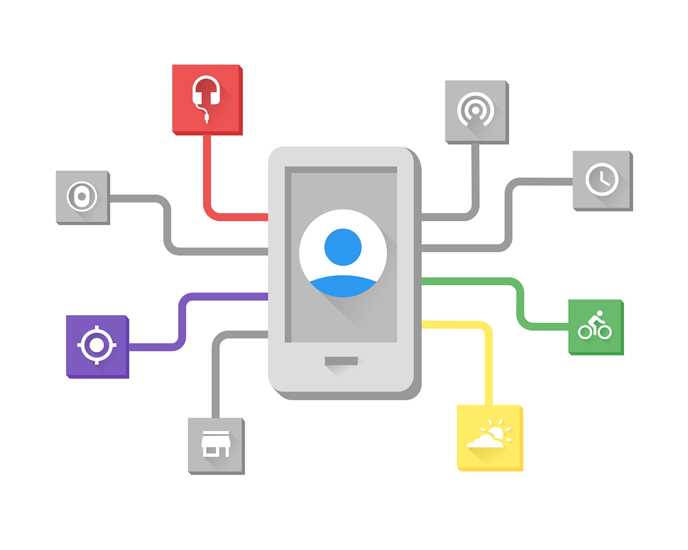
\includegraphics[width=\linewidth]{assets/context_aware.png}
        \end{figure}
    \end{column}
\end{columns}
\end{frame}
\note[itemize]{
\item Con questa espressione si intende un tipo di interazione uomo-macchina che non richiede dei comandi espliciti da parte dell’utente
\item piuttosto utilizza il contesto in cui quest’ultimo agisce come input per l’elaborazione
\item approccio fondamentale per garantire la sicurezza degli utenti durante la guida
}

\begin{frame}{I sensori}
\vspace{0.5cm}
\begin{columns}
    \begin{column}{0.95\textwidth}
        In GeneroCity un sensore è un modulo software che, analizzando il contesto in cui agisce l’utente in uno specifico istante, determina l’azione compiuta da quest’ultimo.
    \end{column}
\end{columns}
\vspace{0.5cm}

\begin{columns}
    \begin{column}{0.15\linewidth}
    \end{column}
    \begin{column}{0.15\linewidth}
        \begin{figure}
            \centering
            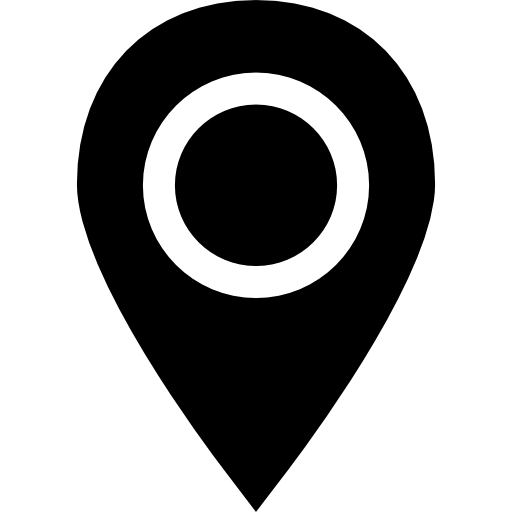
\includegraphics[width=0.7\linewidth]{assets/ic_gps.png}
        \end{figure}
    \end{column}
    \begin{column}{0.15\linewidth}
        \begin{figure}
            \centering
            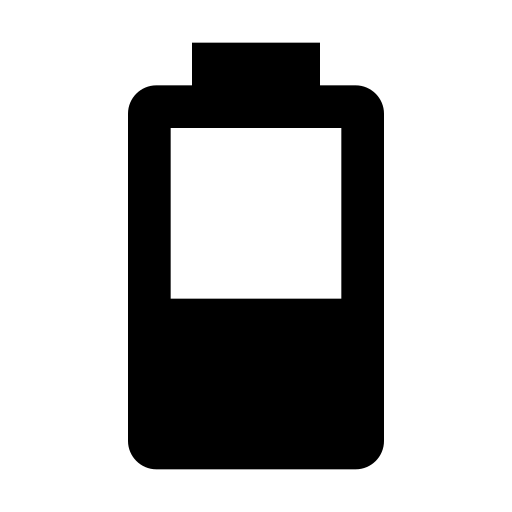
\includegraphics[width=0.8\linewidth]{assets/ic_battery.png}
        \end{figure}
    \end{column}
    \begin{column}{0.15\linewidth}
        \begin{figure}
            \centering
            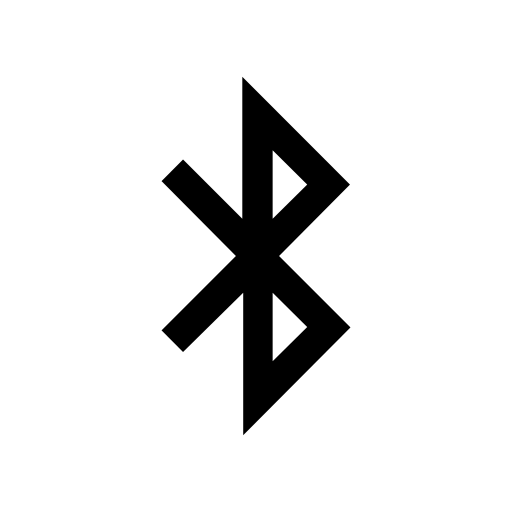
\includegraphics[width=0.9\linewidth]{assets/ic_bluetooth.png}
        \end{figure}
    \end{column}
    \begin{column}{0.15\linewidth}
        \begin{figure}
            \centering
            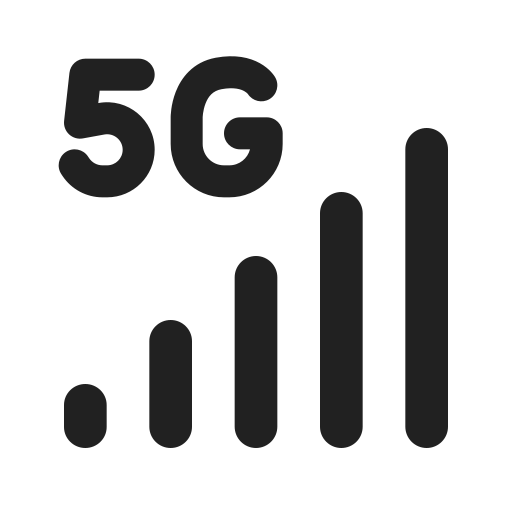
\includegraphics[width=0.8\linewidth]{assets/ic_cell.png}
        \end{figure}
    \end{column}
    \begin{column}{0.15\linewidth}
        \begin{figure}
            \centering
            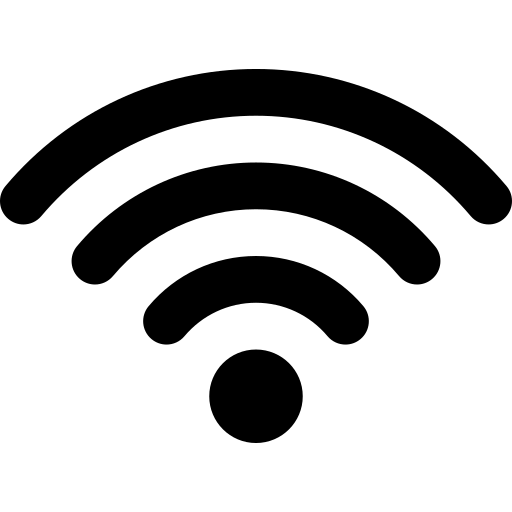
\includegraphics[width=0.8\linewidth]{assets/ic_wifi.png}
        \end{figure}
    \end{column}
    \begin{column}{0.15\linewidth}
    \end{column}

\end{columns}
\end{frame}
\note[itemize]{
\item questo tipo d'interazioni vengono ottenute grazie all’implementazione di appositi moduli software chiamati sensori
\item si occupano di studiare il contesto attraverso l'analisi dei dati riguardanti lo stato del dispositivo
\item ad esempio i dati riguardanti il GPS del dispositivo, la batteria, il WiFi, la linea telefonica o, come per quello da me sviluppato, il Bluetooth
\item scopo: inferire lo stato dell'utente
\item nello specifico se sta guidando o meno
}

\begin{frame}{La confidenza}
Valore $c\in\mathbb{R}$ compreso tra $0$ e $1$:
\begin{itemize}
    \item $c\in[0.0, 0.5)\to$ l'utente non sta guidando
    \item $c=0.5\to$ il sensore non è in grado di inferire lo stato dell'utente
    \item $c\in(0.5, 1.0]\to$ l'utente sta guidando
\end{itemize}
\vspace{1cm}
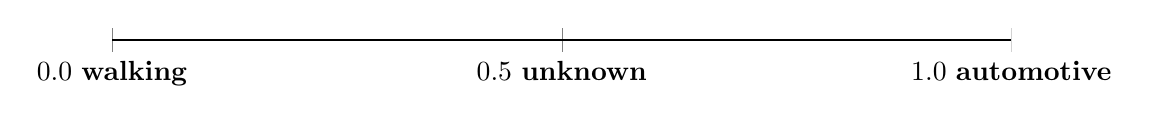
\begin{tikzpicture}
\begin{axis}[
    axis line style=thick,
    axis x line=middle,
    axis y line=none,
    width = 13cm,
    xtick distance=0.5,
    xticklabels={0, $0.0$ \textbf{walking}, $0.5$ \textbf{unknown}, $1.0$ \textbf{automotive}},
    major tick length = 0.3cm,
]
\end{axis}
\end{tikzpicture}
\end{frame}
\note[itemize]{
\item ogni sensore calcola un valore reale compreso tra 0 e 1 detto confidenza 
\item esso rappresenta lo stato dell'utente 
\item quando minore di 0.5 indica lo stato walking, ossia che l'utente non si trova alla guida
\item se uguale a 0.5 denota che il sensore non è in grado di determinare lo stato
\item quando maggiore di 0.5 indica lo stato automotive, ossia che l'utente sta guidando
}

\section{Il sensore Bluetooth}
\note[itemize]{
\item Il mio apporto al progetto GeneroCity è stato quello di realizzare il sensore Bluetooth per l'applicazione Android 
}

\begin{frame}{L'obbiettivo del sensore}
    \vspace{0.5cm}
    Rilevare connessioni Bluetooth con l'autoradio della macchina che l'utente sta guidando.
    \vspace{0.5cm}
    \begin{figure}
        \centering
        
\includegraphics[width=0.5\linewidth]{assets/bt_logo.png}
    \end{figure}
\end{frame}
\note[itemize]{
\item si occupa di riconoscere se i dispositivi connessi allo smartphone dell'utente sono delle autoradio in modo da rilevare quando quest'ultimo sta guidando.
\item per far ciò il sensore ha bisogno di mantenere in memoria il suo stato
}

\begin{frame}{Lo stato del sensore}
\vspace{0.5cm}
\begin{columns}
    \begin{column}{0.5\textwidth}
        \begin{itemize}
            \item<1-> Stato del Bluetooth (acceso/spento)
            \item<2-> Lista dei dispositivi connessi
            \item<3-> Lista delle ultime 10 auto connesse
        \end{itemize}
    \end{column}
\end{columns}
\vspace{0.5cm}
\begin{columns}
    \begin{column}{0.1\linewidth}
    \end{column}
    \begin{column}{0.2\linewidth}
        \begin{figure}
            \centering
            \includegraphics<1->[width=0.6\linewidth]{assets/ic_bt_disabled.png}
        \end{figure}
    \end{column}
    \begin{column}{0.05\linewidth}
    \end{column}
    \begin{column}{0.2\linewidth}
        \begin{figure}
            \centering
            \includegraphics<2->[width=0.8\linewidth]{assets/ic_devices.png}
        \end{figure}
    \end{column}
    \begin{column}{0.05\linewidth}
    \end{column}
    \begin{column}{0.2\linewidth}
        \begin{figure}
            \centering
            \includegraphics<3->[width=0.7\linewidth]{assets/ic_car.png}
        \end{figure}
    \end{column}
    \begin{column}{0.1\linewidth}
    \end{column}
\end{columns}
\note[itemize]{
\begin{itemize}
\item rappresentato da
    \begin{itemize}
        \item un flag che indica se il Bluetooth è acceso o spento
        \item la lista dei dispositivi che sono connessi in quell'istante
        \item la lista delle ultime 10 automobili che sono state connesse
    \end{itemize}
\item questi dati saranno utilizzati per effettuare il calcolo della confidenza
\item lo stato ha bisogno di essere aggiornato ogni qualvolta viene acceso o spento il Bluetooth o viene connesso un dispositivo
\end{itemize}
}
\end{frame}

\begin{frame}{L'ascolto degli eventi di sistema}
\vspace{-0.5cm}
\begin{figure}
    \centering
    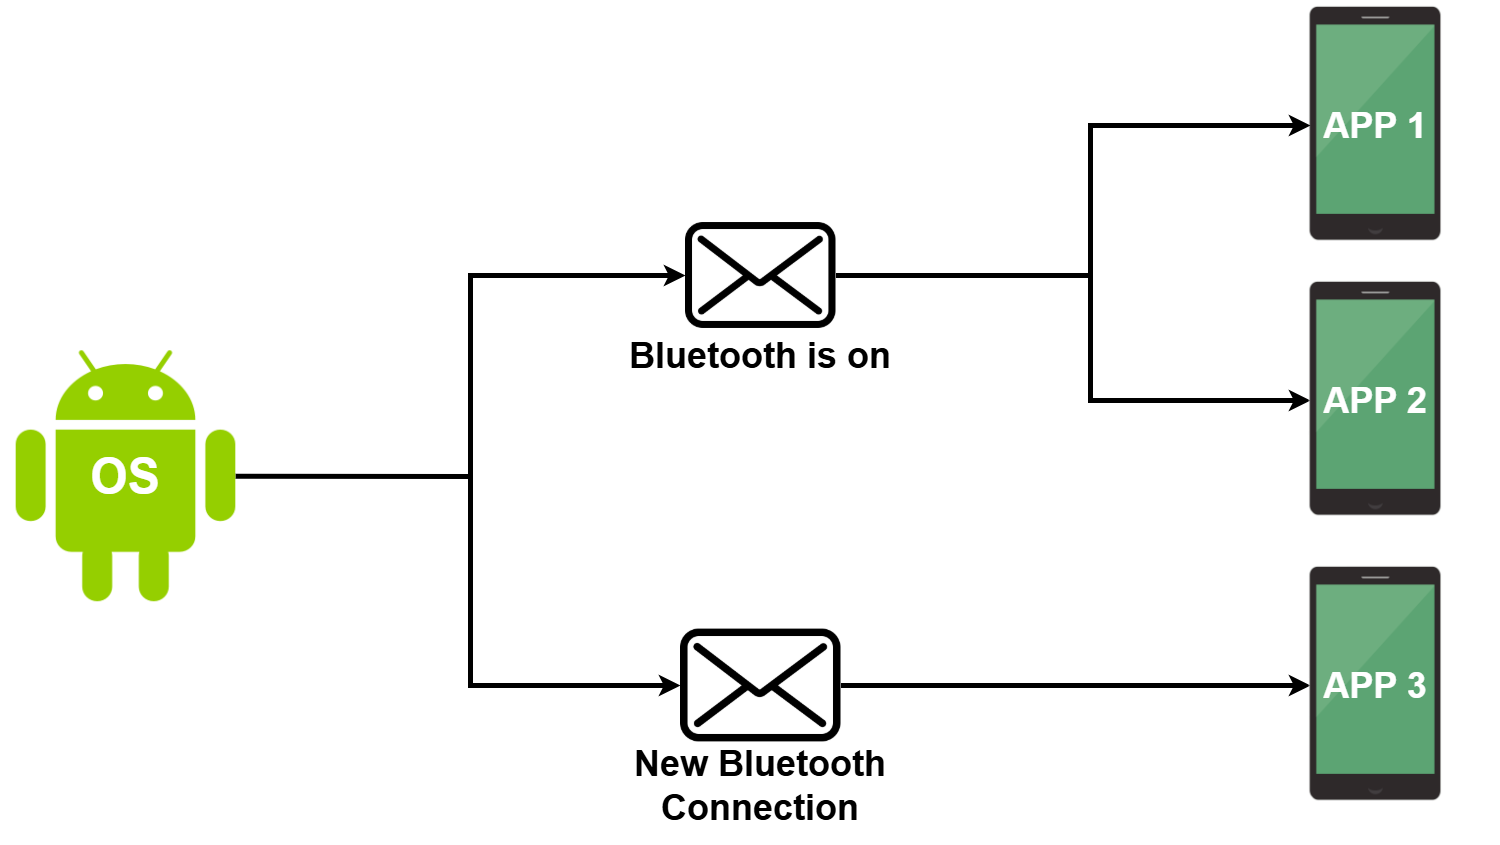
\includegraphics[width=0.9\linewidth]{assets/system_broadcast.png}
\end{figure}
\end{frame}
\note[itemize]{
\item a tale scopo vengono ascoltati degli eventi di sistema
\item infatti in Android le applicazioni possono registrarsi per essere notificate dal sistema operativo quando degli specifici eventi di sistema accadono
\item in questo caso al sensore interessano solamente gli eventi relativi al Bluetooth, più precisamente
\begin{itemize}
    \item l'accensione e lo spegnimento del bluetooth
    \item la connessione di un dispositivo bluetooth
\end{itemize}
}

\begin{frame}{Il rilevamento della connessione di un'automobile}
\begin{figure}
    \centering
    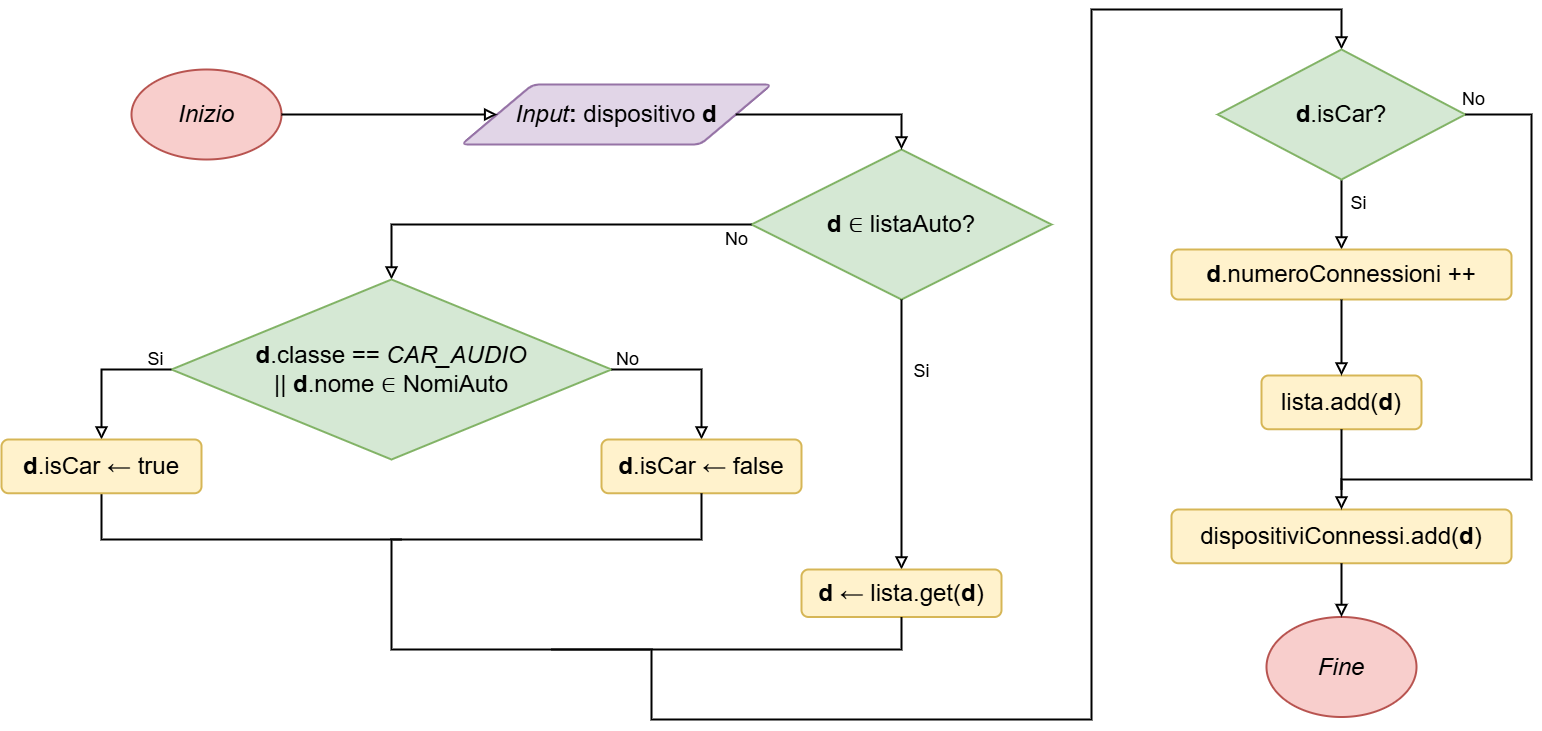
\includegraphics[width=\linewidth]{assets/algoritmo.png}
\end{figure}
\end{frame}
\note[itemize]{
\item nello specifico quando il sensore viene notificato di una nuova connessione sarà eseguito il seguente algoritmo per verificare se il dispositivo connesso è un'automobile o meno 
\item prima di tutto viene verificato se il dispositivo è già presente tra le macchine salvate (tramite indirizzo mac)
\begin{itemize}
    \item se si verrà prelevato dalla lista in quanto memorizza il numero di connessioni effettuate in precedenza
\end{itemize}
\item in caso contrario controlla se si tratta di un'auto:
\begin{itemize}
    \item viene controllato se utilizza la classe specifica per le autoradio bluetooth oppure se il nome del dispositivo è quello di un brand o modello di auto, se si flag isCar=true
    \item false
\end{itemize}
\item successivamente, nel caso in cui il dispositivo connesso è un'auto, indipendentemente dal fatto che era già presente, incrementa di uno il contatore delle sue connessioni e viene salvato nella lista delle macchine (sovrascrivendo il vecchio se presente)
\item infine viene salvato il dispositivo alla lista dei dispositivi connessi
}

\section{Il calcolo della confidenza}
\note[itemize]{
\item ogni volta che lo stato del sensore cambia a seguito di un evento di sistema, viene calcolata la confidenza in modo da aggiornare lo stato dell'utente di conseguenza
\item in particolare
}

\begin{frame}{La confidenza restituita dal sensore Bluetooth}
\begin{itemize}
    \item<1-> Bluetooth spento $\to c=0.5$
    \item<2-> Nessun dispositivo connesso $\to c=0.0$
    \item<3-> Nessuna automobile tra i dispositivi connessi $\to c=0.1$
    \item<4-> Automobile connessa  $\to c\in[0.75, 1.0]$
\end{itemize}
\vspace{1.5cm}
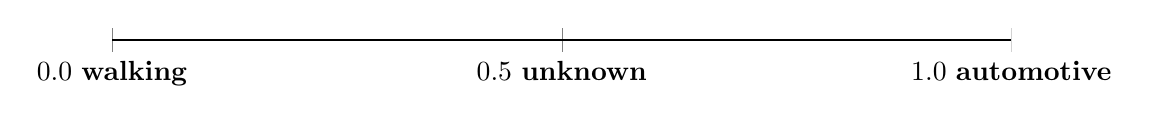
\begin{tikzpicture}
\begin{axis}[
    axis line style=thick,
    axis x line=middle,
    axis y line=none,
    width = 13cm,
    xtick distance=0.5,
    xticklabels={0, $0.0$ \textbf{walking}, $0.5$ \textbf{unknown}, $1.0$ \textbf{automotive}},
    major tick length = 0.3cm,
]
\end{axis}
\end{tikzpicture}
\note{
\begin{itemize}
    \item Se al momento del ricalco il Bluetooth è spento $\to c=0.5$ in quanto non può stimare lo stato
    \item Se invece è acceso ma non c'è nessun dispositivo connesso $\to c=0.0$ sicuramente non connessa un macchina
    \item Altrimenti se ci sono dispositivi connessi ma nessuno di essi è un'auto $\to c=0.1$ dato che potrebbero essere presenti automobili non rilevate correttamente
    \item Se invece un'automobile è connessa $\to c\in[0.75, 1.0]$ proporzionale al numero di connessioni
\end{itemize}
}
\end{frame}

\begin{frame}{Confidenza proporzionale al numero di connessioni}
\begin{columns}
    \begin{column}{0.3\textwidth}
        \begin{figure}
            \centering
            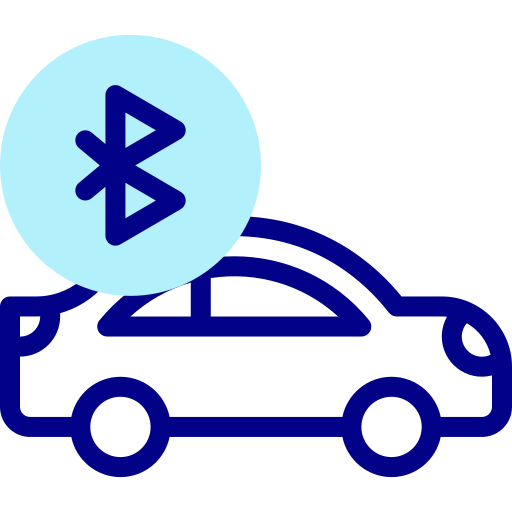
\includegraphics[width=\linewidth]{assets/car-bluetooth.png}
        \end{figure}
    \end{column}
    \begin{column}{0.6\textwidth}
        \begin{itemize}
            \item Il sensore deve riconoscere quando l'utente sta guidando e non sia un passeggero
            \item Si basa sul numero di connessioni effettuate con la stessa auto
            \item Più è un'auto usata frequentemente più è probabile che l'utente sia alla guida
        \end{itemize}
    \end{column}
\end{columns}
\end{frame}
\note[itemize]{
\item importante sensore sia in grado di riconoscere quando l’utente si trova effettivamente alla guida e non sia un passeggero
\item per discernere questi due casi si è scelto di basarsi sul numero di connessioni effettuate verso la stessa auto
\item inferendo che, se essa è molto utilizzata, si tratti di un'auto dell’utente e che quindi egli stia guidando
}

\begin{frame}{L'incremento esponenziale della confidenza}
\vspace{0.5cm}
\begin{tikzpicture}
\begin{axis}[
    axis lines = left,
    width = 13cm,
    height = 6cm,
    xmax=15,
    xlabel=Numero di connessioni,
    xtick={0,...,16},
    ymax=1,
    ylabel=Confidenza,
    ymajorgrids=true
]
  \addplot[
        maincolor,
        ultra thick,
        domain= 1:15,
        samples=100
    ] {0.75 + 0.0025 * (1.4^(x-1) -1)};
\end{axis}
\end{tikzpicture}
\end{frame}
\note[itemize]{
\item Anzitutto si è scelto un approccio lineare, ovvero aumentando la confidenza di un valore costante ad ogni connessione da parte della stessa vettura
\item  è emerso che in situazioni di utilizzo sporadico di un automobile come passeggero, la confidenza restituita fosse troppo elevata portando a falsi positivi
\item si è quindi deciso di utilizzare una funzione esponenziale in modo da incrementare leggermente la confidenza per le prime connessioni, mentre per un numero più elevato restituire una confidenza più alta.
\item nello specifico alla prima connessione viene restituito 0.75 ed il valore rimarrà sotto lo 0.8 fino alla decima connessione per poi aumentare più velocemente fino alla quindicesima connessione per cui verrà restituito 1 così come per tutte le successive
\item Questo approccio si è rivelato più affidabile nei test successivi
}

\begin{frame}[containsverbatim]{L'invio dei dati al server}
\vspace{0.25cm}
\begin{figure}
    \centering
    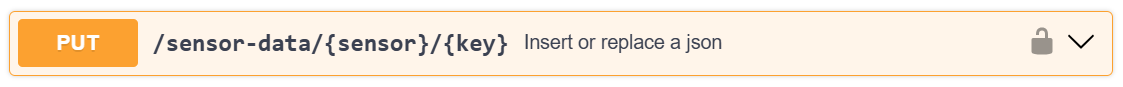
\includegraphics[width=0.8\linewidth]{assets/endpoint.png}
\end{figure}
% \vspace{-0.25cm}
\begin{columns}
\begin{column}{0.6\textwidth}
\begin{block}{Esempio di body inviato dal sensore}
\begin{Verbatim}[fontsize=\tiny]
{
   "action":"automotive",
   "confidence":0.75436,
   "data":{
      "bluetooth_enabled":true,
      "connected":[
         {
            "alias":"My Car",
            "bluetooth_class":"Handsfree",
            "connection_count":4,
            "device_name":"Fiat Punto",
            "is_car":true
         }
      ]
   },
   "datetime":"2024-10-21T15:43:24.525+02:00"
}
\end{Verbatim}
\end{block}
\end{column}
\end{columns}
\end{frame}
\note[itemize]{
\item ogni sensore quando il suo stato  cambia e confidenza ricalcolata
\item invia una richiesta HTTP ad un apposito endpoint esposto dal server
\item nel body richiesta si serializzano ...
\item questi dati vengono raccolti per allenare un modello di machine learning 
\begin{itemize}
    \item attualmente in sviluppo
    \item scopo: determinare lo stato dell'utente basandosi sulla confidenza calcolata da ogni sensore
\end{itemize}
}

% Se sono corto con i tempi aggiungere slide sul testing

\backmatter
\note[itemize]{
\item \textbf{Possibili domande}:
\item Testing:
    \begin{itemize}
        \item circa una 50 di test
        \item accendendo la macchina e connettendola al telefono
        \item verificando con un interfaccia grafica da me realizzata che veniva rilevata correttamente la connessione di una macchina
        \item e che la confidenza restituita fosse coerente con il numero di connessioni
    \end{itemize}
}
\end{document}
